\section{Results} \label{resultsSec}
  \vspace{-15pt}
  \begin{figure}[H]
      \centering
      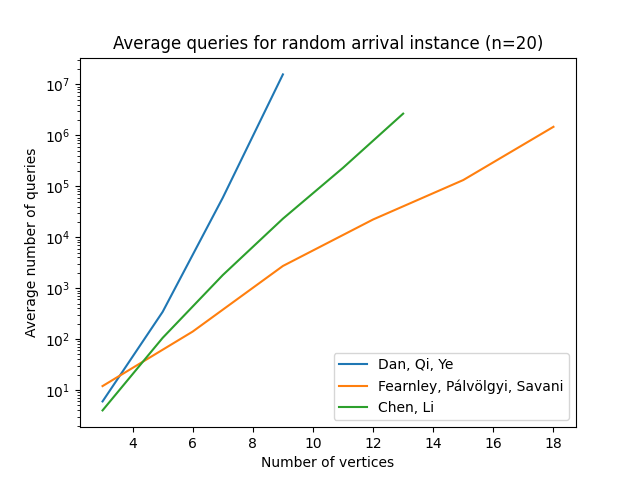
\includegraphics[width=2.6in]{plots/arrival_queries.png}
      \centering
      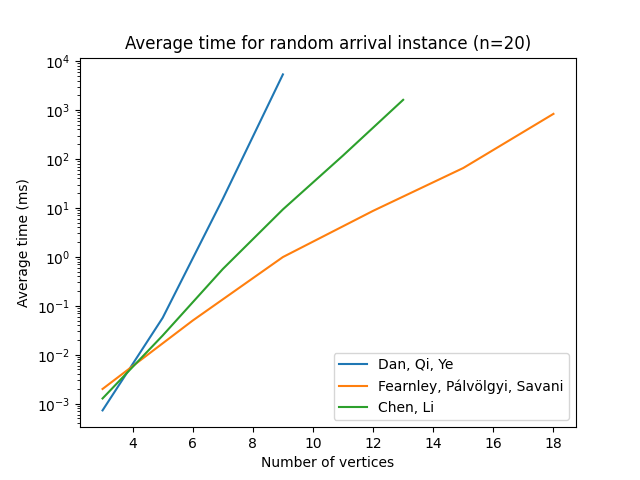
\includegraphics[width=2.6in]{plots/arrival_time.png}
      \caption{\cref{arrMainTest}. The binary search style algorithms take an approximately
      exponential time and amount of queries on random arrival instances in practice. FPS is the fastest.} \label{arrivalMainPlot}
  \end{figure}
  \vspace{-22pt}
  \begin{figure}[H]
      \centering
      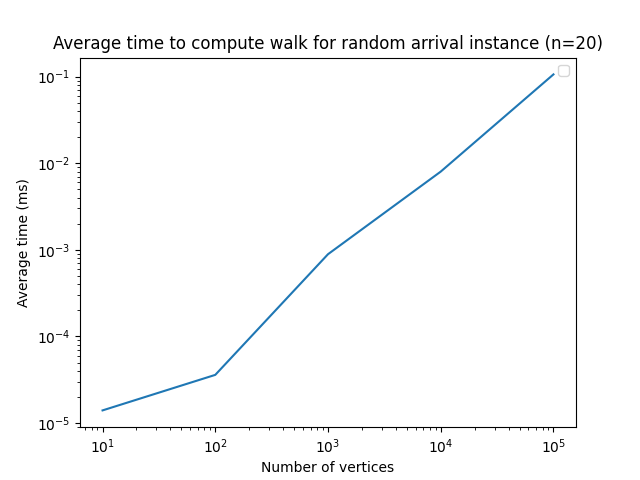
\includegraphics[width=2.6in]{plots/arrival_steps.png}
      \centering
      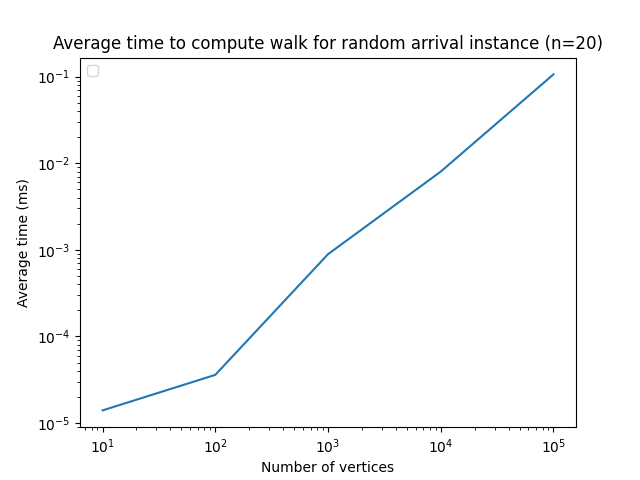
\includegraphics[width=2.6in]{plots/arrival_wtime.png}
      \caption{\cref{arrWalkTest}. Time and number of steps taken to simulate the arrival
      walk scales roughly linearly with the size of the problem in practice. Simulating
      the walk is vastly more performant than binary search style algorithms for random arrival instances.} \label{arrivalWalkPlot}
  \end{figure}
  \vspace{-22pt}
  \begin{figure}[H]
      \centering
      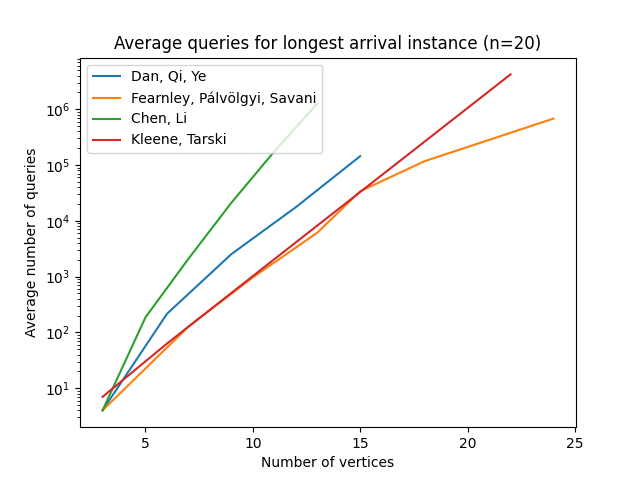
\includegraphics[width=2.6in]{plots/arrival_long_queries.png}
      \centering
      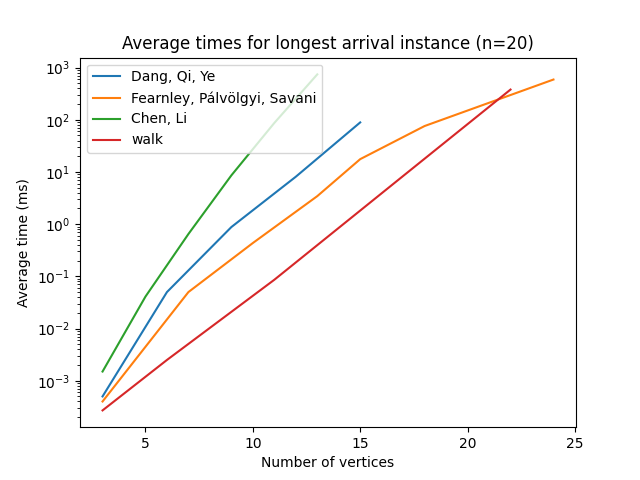
\includegraphics[width=2.6in]{plots/arrival_long_times.png}
      \caption{\cref{longArrivalTest}. On the arrival instance with the longest possible walk as in \cref{expLongArrival},
      FPS achieves similar performance to just simulating the walk.} \label{arrivalLongPlot}
  \end{figure}
  
  \vspace{-22pt}
  \begin{figure}[H] 
      \centering
      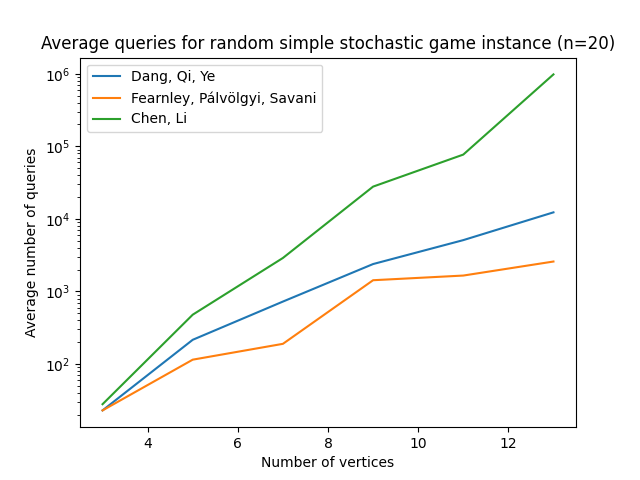
\includegraphics[width=2.6in]{plots/simple_queries.png}
      \centering
      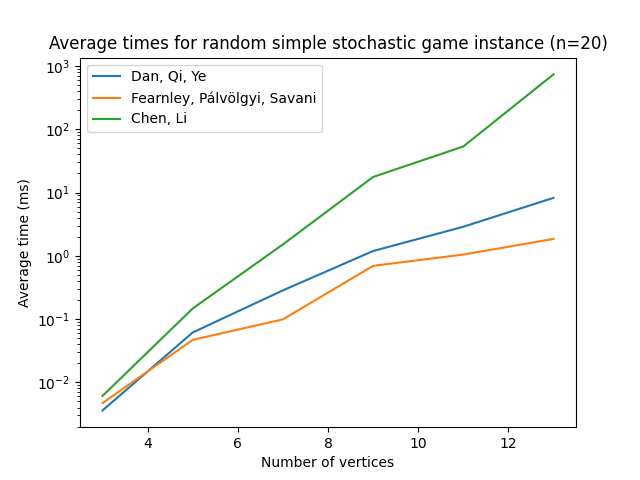
\includegraphics[width=2.6in]{plots/simple_times.png}
      \caption{\cref{ssgMainTest}. The binary search style algorithms take an approximately exponential
      amount of time and queries in the number of nodes
      to solve random simple stochastic games with fixed stopping probability
      and approximation constant.} \label{simpleMainPlot}
  \end{figure}
  \vspace{-20pt}
  \begin{figure}[H]
      \centering
      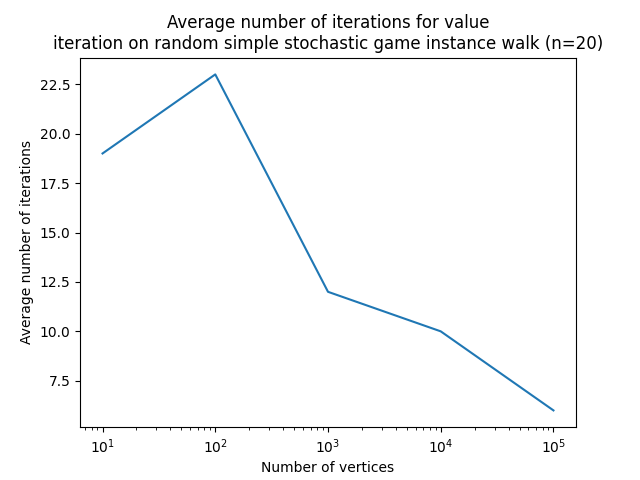
\includegraphics[width=2.6in]{plots/simple_iterations.png}
      \centering
      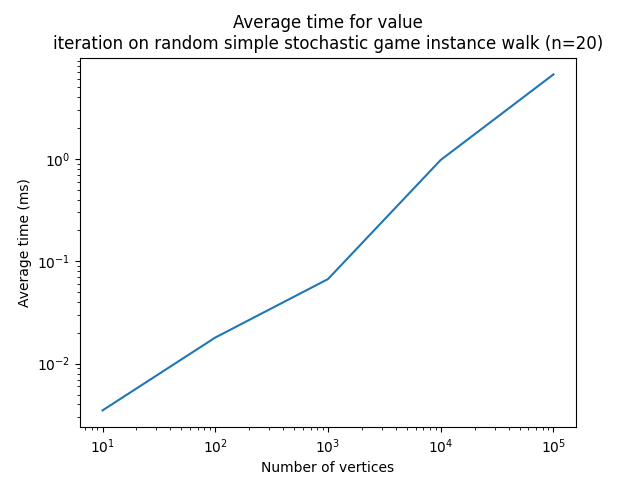
\includegraphics[width=2.6in]{plots/simple_iter_time.png}
      \caption{\cref{ssgMainTest} cont. Value iteration takes approximately linear time and oddly downward scaling
      queries in the number of nodes
      to solve random simple stochastic games with fixed stopping probabilities and approximation constant.
      It is drastically more performant than
      the binary search style algorithms.} \label{simpleWalkPlot}
  \end{figure}
  \vspace{-20pt}
  \begin{figure}[H]
      \centering
      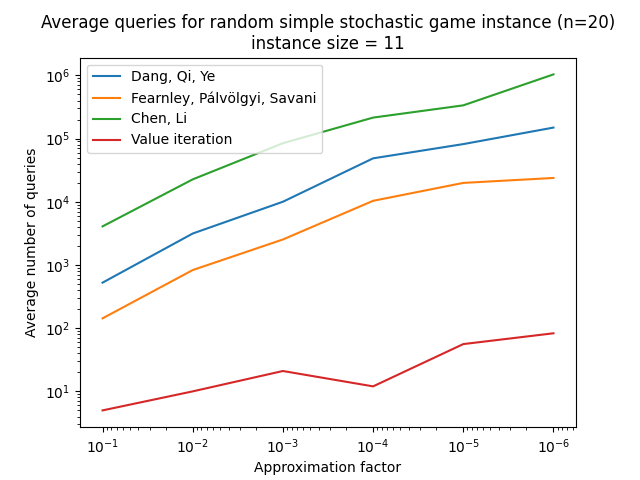
\includegraphics[width=2.6in]{plots/simple_eps_queries.png}
      \centering
      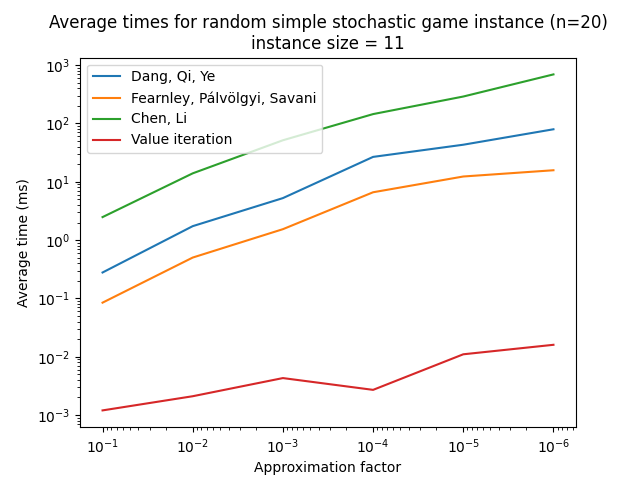
\includegraphics[width=2.6in]{plots/simple_eps_times.png}
      \caption{\cref{ssgApproxTest}. Value iteration easily outperforms the binary search style algorithms
      in solving simple stochastic games with a fixed number of nodes and varying approximation constant.
      Of the binary search algorithms, FPS is the most performant.} \label{simpleApproxPlot}
  \end{figure}
  \vspace{-20pt}
  \begin{figure}[H]
      \centering
      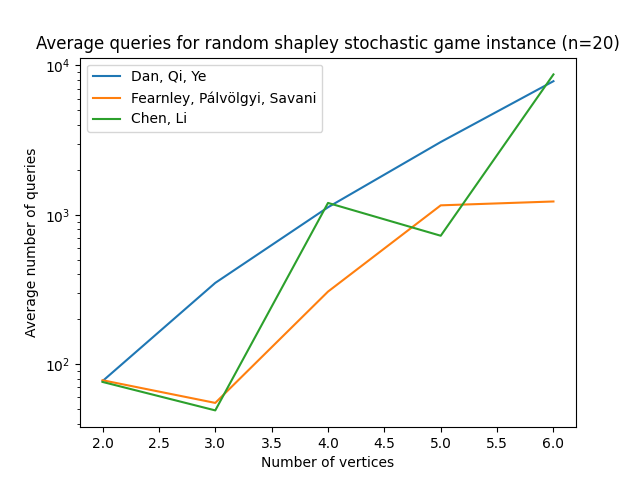
\includegraphics[width=2.6in]{plots/shapley_queries.png}
      \centering
      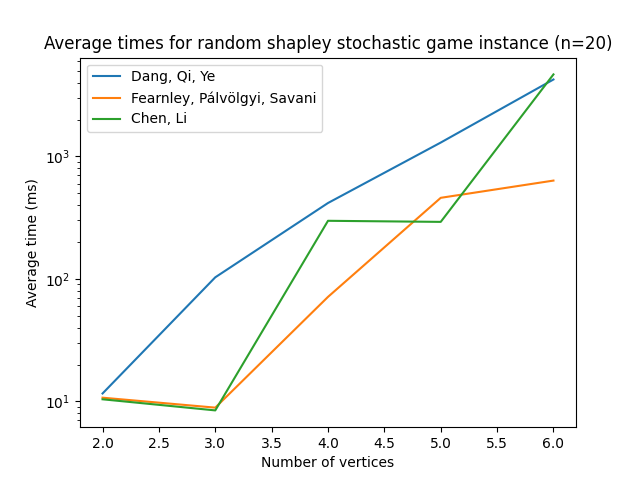
\includegraphics[width=2.6in]{plots/shapley_times.png}
      \caption{\cref{shapleyMainTest}. The binary search style algorithms take an approximately exponential
      time in solving random shapley's stochastic games. FPS and CL see similar performance for the
      sizes tested.} \label{shapleyMainPlot}
  \end{figure}
  \vspace{-20pt}
  \begin{figure}[H]
      \centering
      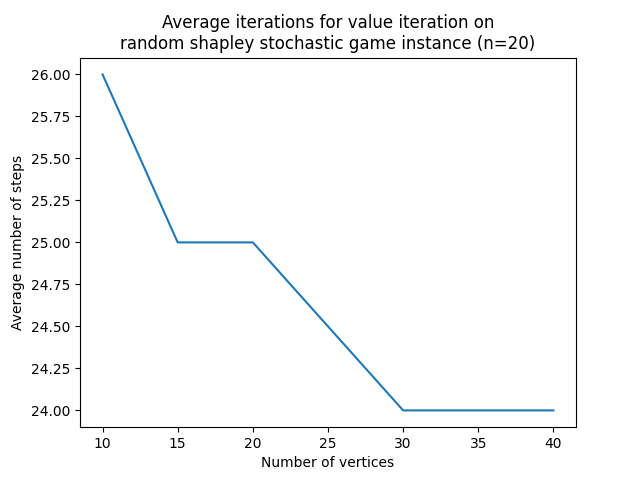
\includegraphics[width=2.6in]{plots/shapley_iterations.png}
      \centering
      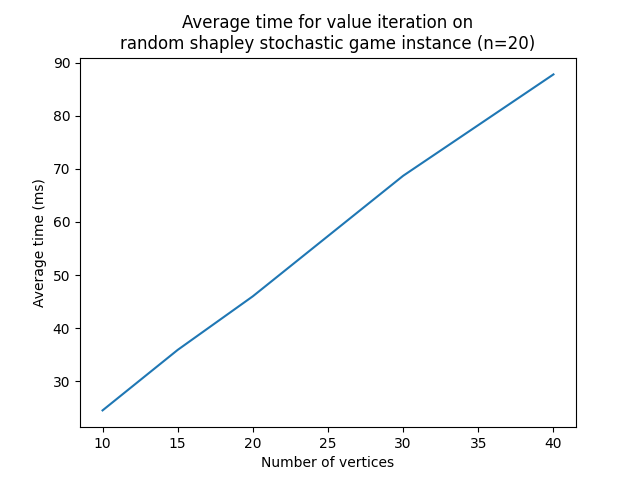
\includegraphics[width=2.6in]{plots/shapley_iter_time.png}
      \caption{\cref{shapleyMainTest} cont. Value iteration takes approximately linear time
      and a close to constant number of queries to solve shapley's stochastic games on the sizes tested.
      It is much more performant than the binary search style algorithms. The constant factor involved in
      computing the monotone function is significant and results in longer solves than $\arr$ and simple stochastic games.} \label{shapleyWalkPlot}
  \end{figure}
  \vspace{-20pt}
  \begin{figure}[H]
      \centering
      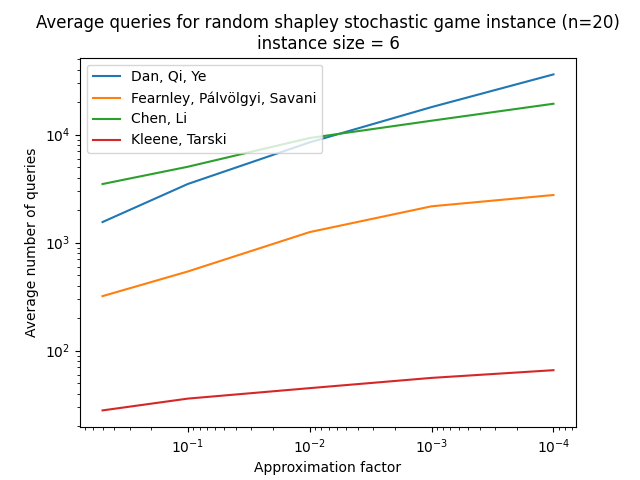
\includegraphics[width=2.6in]{plots/shapley_eps_queries.png}
      \centering
      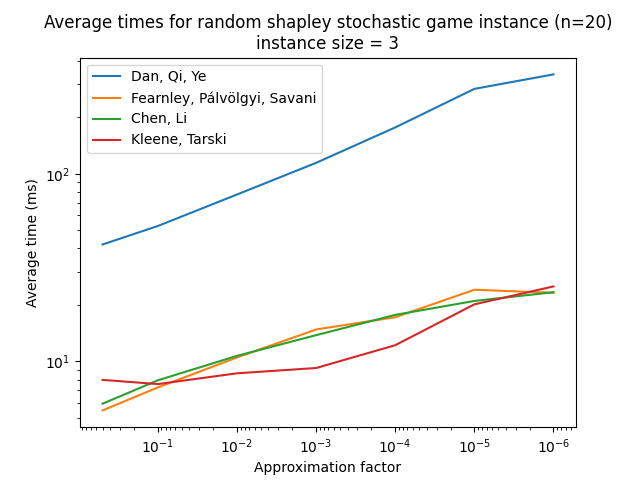
\includegraphics[width=2.6in]{plots/shapley_eps_times.png}
      \caption{\cref{shapleyApproxTest}. Value iteration outperforms the binary search style algorithms in solving
      shapley's stochastic games with fixed size and varying approximation constant.} \label{shapleyApproxPlot}
  \end{figure}
  All data used in these plots can be found \href{https://github.com/angusjoshi/tarski/blob/main/src/analysis/makePlots.py}{here}.
